\documentclass[]{article}

% math packages
\usepackage{amsmath}
\usepackage{amsthm}
\usepackage{bm}

% including graphics
\usepackage{graphicx}
\graphicspath{ {./images/} }

% drawing graphs
\usepackage{tikz-cd}
\usepackage{tikz}
\usetikzlibrary{shapes.geometric, arrows}
\tikzstyle{startstop} = [rectangle, rounded corners, minimum width=3cm, minimum height=1cm,text centered, draw=black, fill=red!10]
\tikzstyle{arrow} = [thick,->,>=stealth]

% some useful shortcuts
\DeclareMathOperator*{\argmax}{argmax}
\newcommand{\indep}{\perp\!\!\!\!\perp}
\newcommand{\blambda}{{\bm{\lambda}}}
\newcommand{\btheta}{{\bm{\theta}}}
\newcommand{\bpsi}{{\bm{\psi}}}

\newcommand{\by}{\mathbf{y}}

%opening
\title{Multisite power writeup}
\author{Jonathan Che}

\begin{document}
	
\maketitle

%\begin{abstract}
%\end{abstract}


\section{Introduction}

With many multisite trials, researchers are often still interested in individual site-level treatment effects.
While there is an extensive literature on power analyses for the overall average treatment effect, cross-site variation, and fixed effects in multisite trials (e.g., Raudenbush \& Liu 2000, many others...), less attention has been paid to inferences for random effects.
Since researchers typically model site-level treatment effects as random effects, the power of a particular study design to detect these effects remains unclear.
In this simulation study, we conduct power analyses for site-level treatment effects in multisite trials.


\section{Data-generating process}

We use the \texttt{blkvar} package in R to simulate multisite trials data, according to the model:
\begin{align*}
	Y_{ij} &= \alpha_j + \tau_j Z_{ij} + \epsilon_{ij} \\
	\alpha_j &= 0 + u_{0j} \\
	\tau_j &= \tau + u_{1j} \\
	\begin{pmatrix}
		u_{0j} \\ u_{1j}
	\end{pmatrix} &\sim N(
	\begin{pmatrix}
		0 \\ 0
	\end{pmatrix}, 
	\begin{bmatrix}
		ICC & 0 \\ 0 & 0.3
	\end{bmatrix}) \\
	\epsilon_{ij} &\sim N(0, 1-ICC)
\end{align*}
We assume that the treatment proportion in each site is $p=0.5$.
In practice, we round $\tau_j$ to the nearest 0.05 before sampling individual responses so that we can have precise site-effect bins for our visualizations.

The user-specified parameters are:
\begin{itemize}
	\item $\bar{n}$: the average number of students per site
	\item $J$: the total number of sites
	\item $ICC$: the variance of the site intercepts
	\item $\tau$: the overall average treatment effect
\end{itemize}
We fix $Var(Y(0)) = 1$, so that all units are effect-size units and $ICC = \frac{Var(\alpha_i)}{Var(\alpha_i) + Var(\epsilon_{ij})} = Var(\alpha_i)$.
In our simulations, we use: $\bar{n} = 25, 50, 75, 100$; $J = 20$; $ICC = 0, 0.3, 0.6, 0.9$; and $\tau = 0.01, 0.2, 0.5, 0.8$.

Note: was running simulations incorrectly, fixed now! 
Now we have $ICC = \frac{Var(\alpha_i)}{Var(\alpha_i) + Var(\epsilon_{ij})} = Var(\alpha_i)$ as desired.


\section{Results}

Results are as expected.
Power increases as the informativeness of the site data increases, i.e., as $\bar{n}$ and $ICC$ increase.
MLM shrinkage increases rejection rates when $\tau$ is high and site information is low, which increases both the power and the type-I error rate.
For most settings, however, using a multilevel model does not seem to improve power for one-tailed tests for single sites, when compared to simply running a t-test on that site.


\subsection{MLM power analyses}

In this section, we show the power for MLM models to detect positive treatment effects at individual sites, so each multisite trial involves $J$ tests for $H_0: \tau_j \leq 0$.
We simulate multisite trial data and run \texttildelow2000 analyses at $\alpha = 0.1$ to determine power.

Figure \ref{fig:power_plot} shows the power under various simulation settings, plotted against the true ATE for the site.
As mentioned before, we round the simulated true ATE values $\tau_j$ to the nearest 0.05 before generating student data, so the x-axis in Figure \ref{fig:power_plot} uses the rounded $\tau_j$ values.
The dashed lines are at $\alpha = 0.1$ and $0.80$; ideally, the power curve would approximately follow a step function along the dashed lines, with a rejection rate less than 0.1 for true ATE values less than 0, and a rejection rate over 0.8 for true ATE values greater than 0.

We see that as $\bar{n}$ and $ICC$ increase, the power curve approaches the desired step function, as expected.
We also note that MLM shrinkage has a strong effect when information is low (i.e., $\bar{n}$ and/or $ICC$ are low): for high values of $\tau$, the $\tau_j$ estimates are pooled upward, which increases power across all $\tau_j$ values.
This increase in power, however, also results in an elevated type-I error rate for the sites with $\tau_j < 0$.

\begin{figure}[ht]
	\centering
	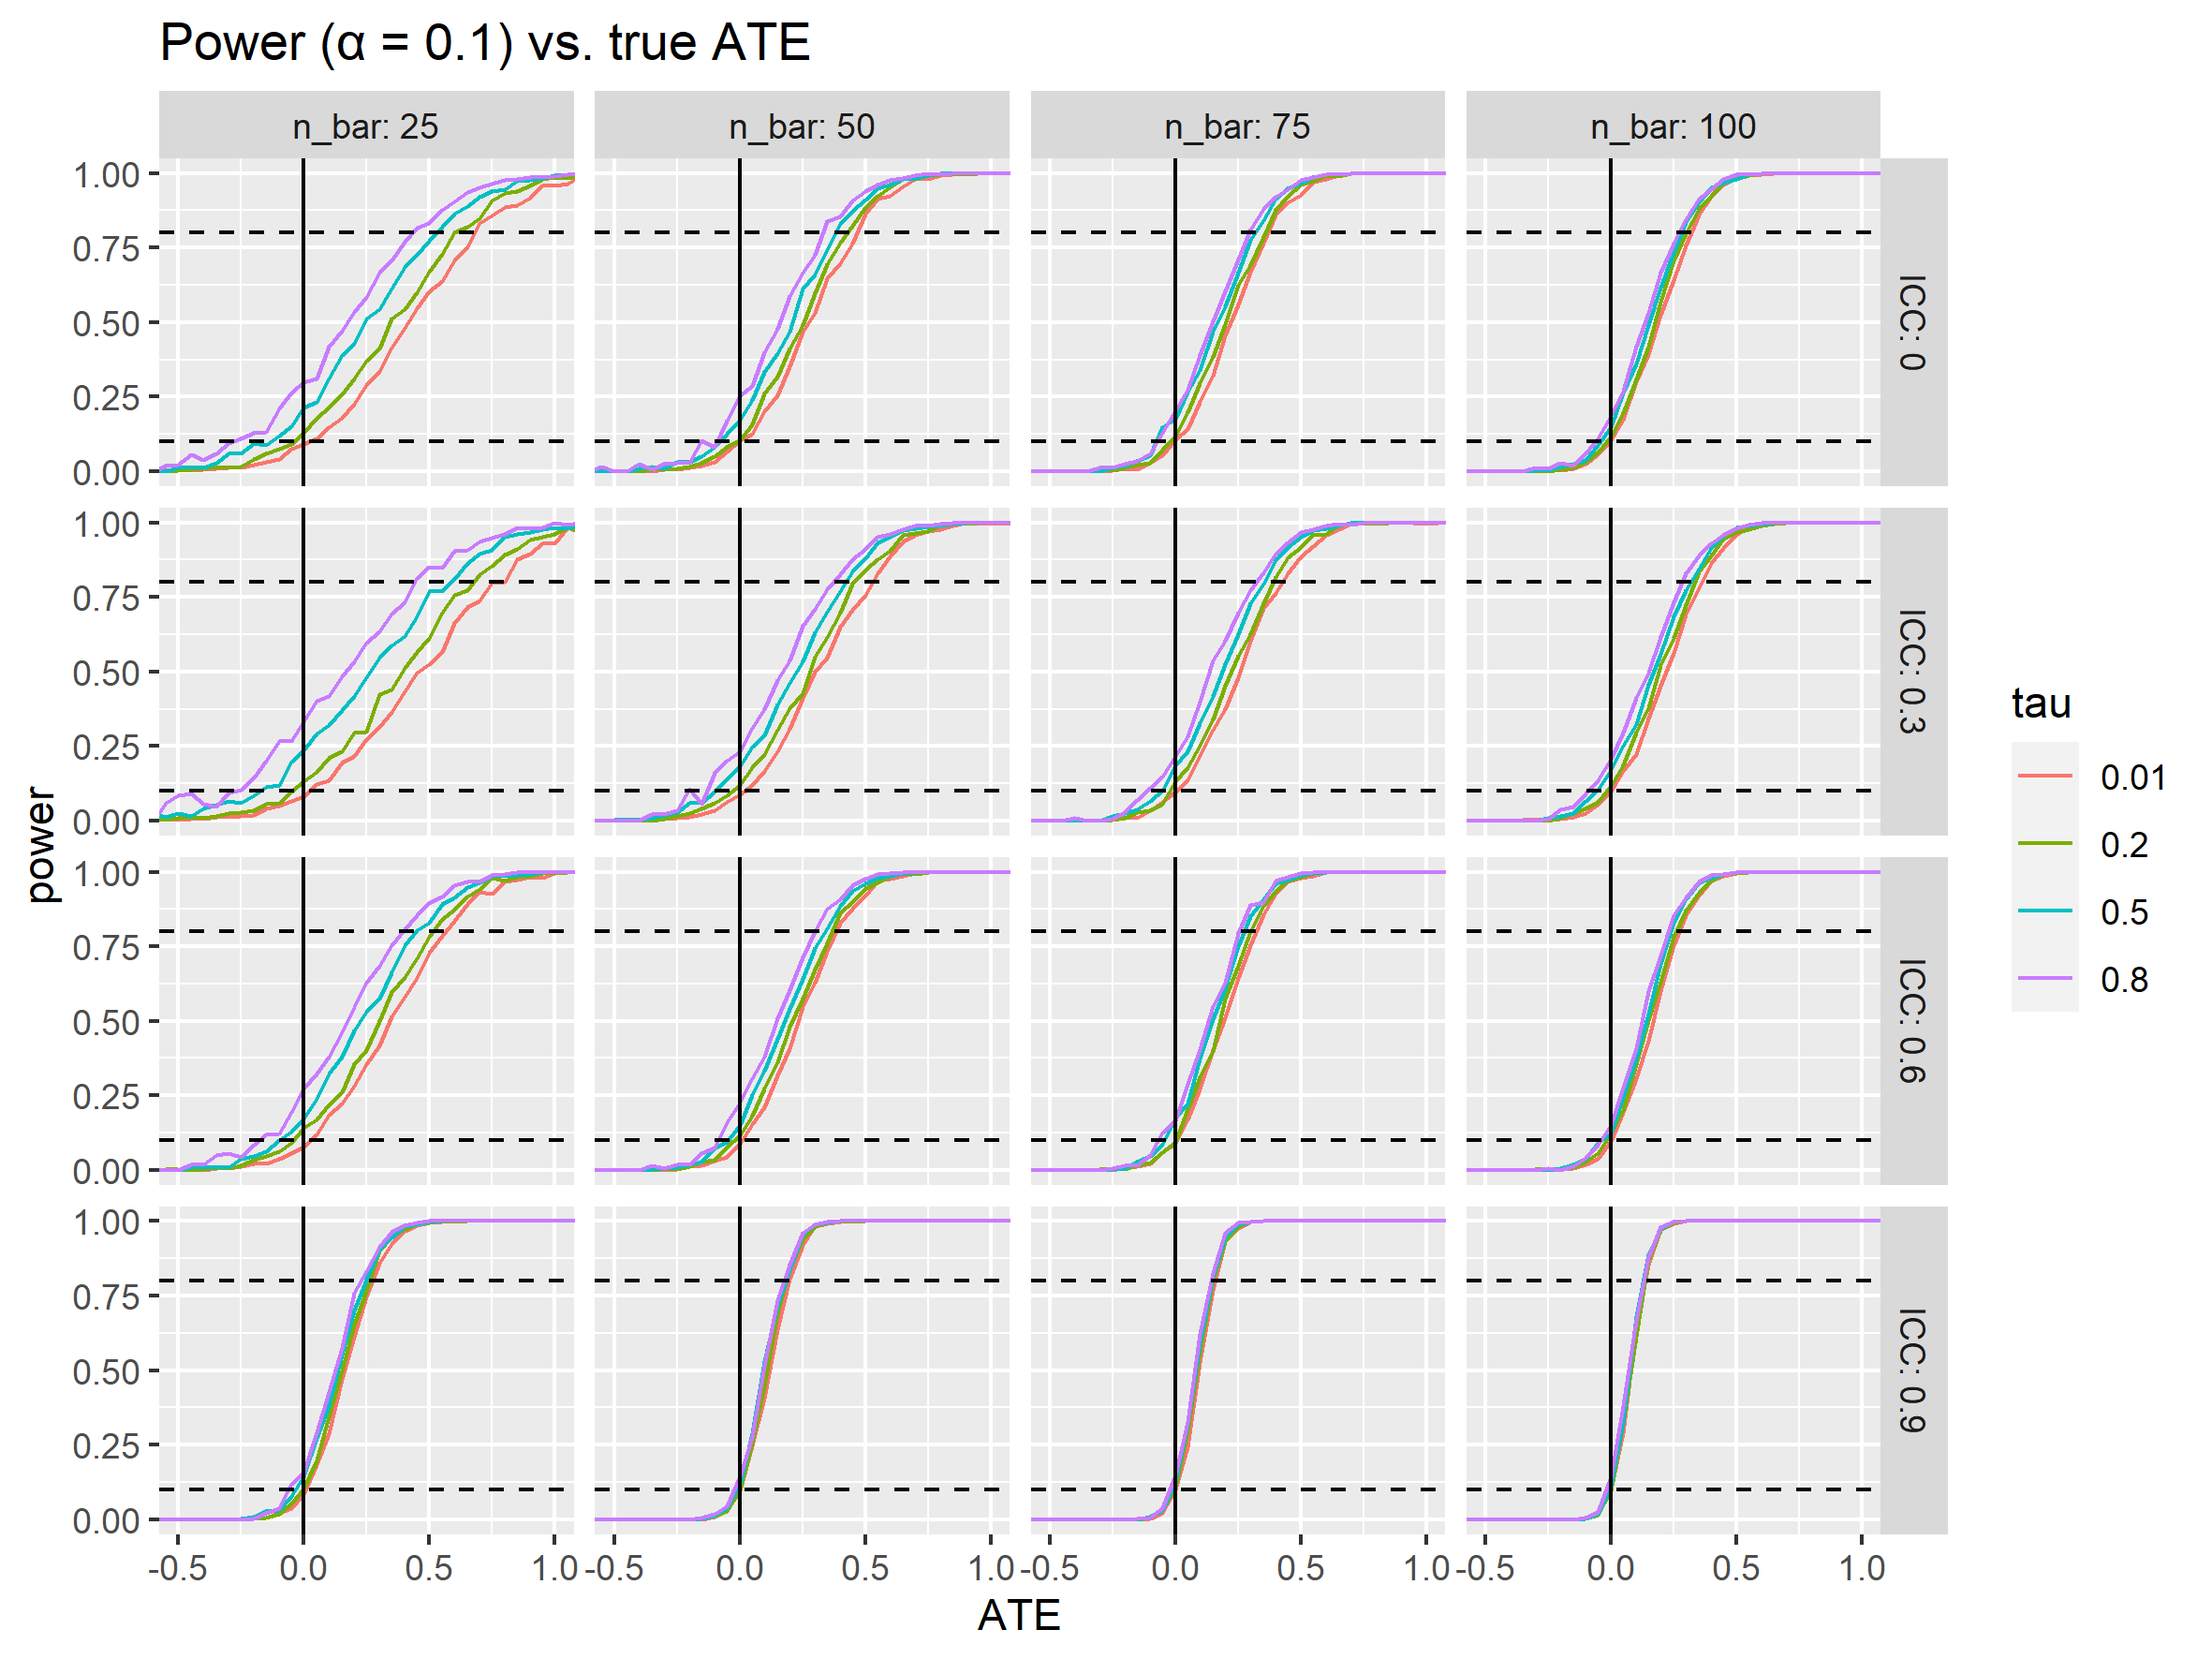
\includegraphics[width=\textwidth]{power_plot}
	\caption{Plot of power (at $\alpha = 0.1$) vs. true site ATE}
	\label{fig:power_plot}
\end{figure}

In Figure \ref{fig:power_plot_ATE02}, we only examine the sites for which $\tau_j = 0.2$, i.e., sites with a moderate effect size that we would hope to be able to detect.
We note that in all but the most extreme $ICC$ setting, we fail to achieve a power of 0.8.

\begin{figure}[ht]
	\centering
	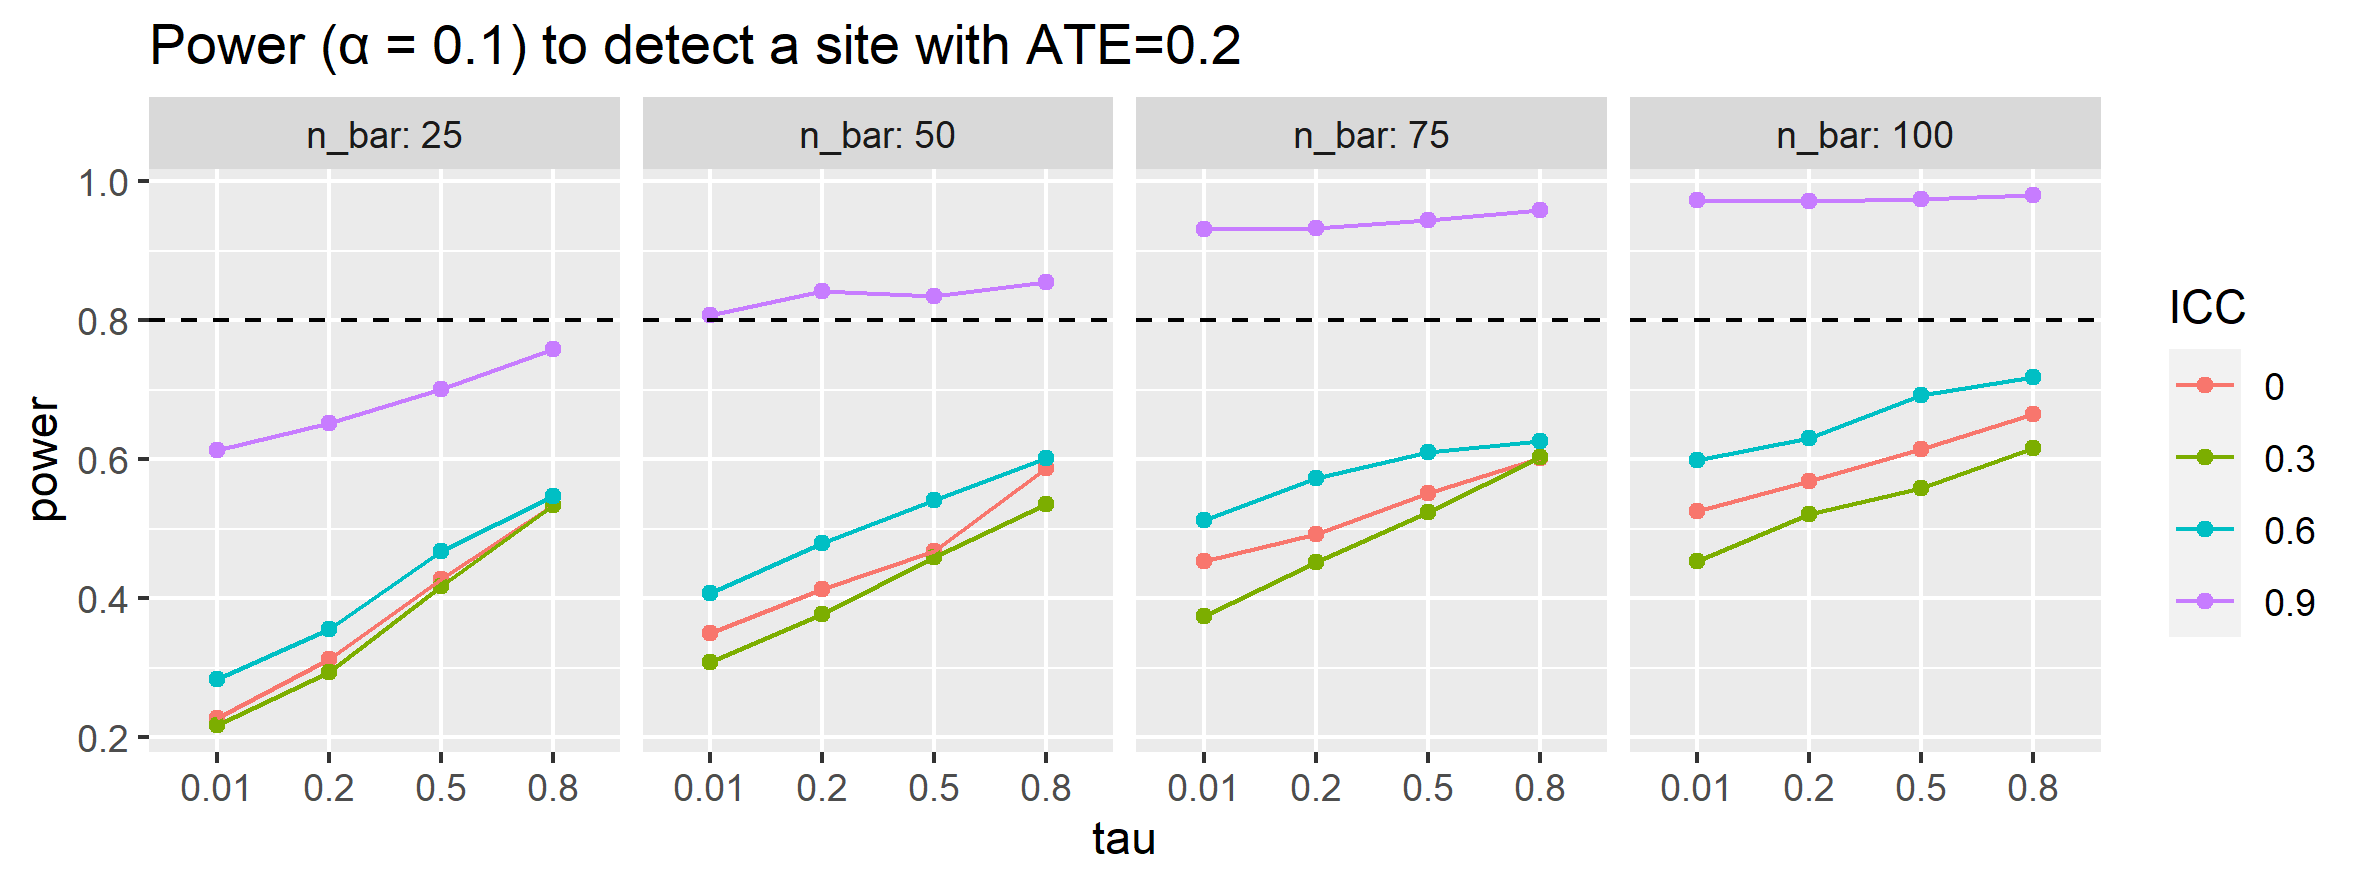
\includegraphics[width=\textwidth]{power_plot_ATE02}
	\caption{Plot of power (at $\alpha = 0.1$) vs. true site ATE}
	\label{fig:power_plot_ATE02}
\end{figure}

Finally, in Figure \ref{fig:power_plot_ATE02_dens}, we again view just the sites for which $\tau_j = 0.2$, but now we visualize the density curves of the estimated $\hat{\tau}_j$ values under various simulation settings.
Again, we note how shrinkage pulls the density curves to the right in the low-information settings, but not in the high-information settings.

\begin{figure}[ht]
	\centering
	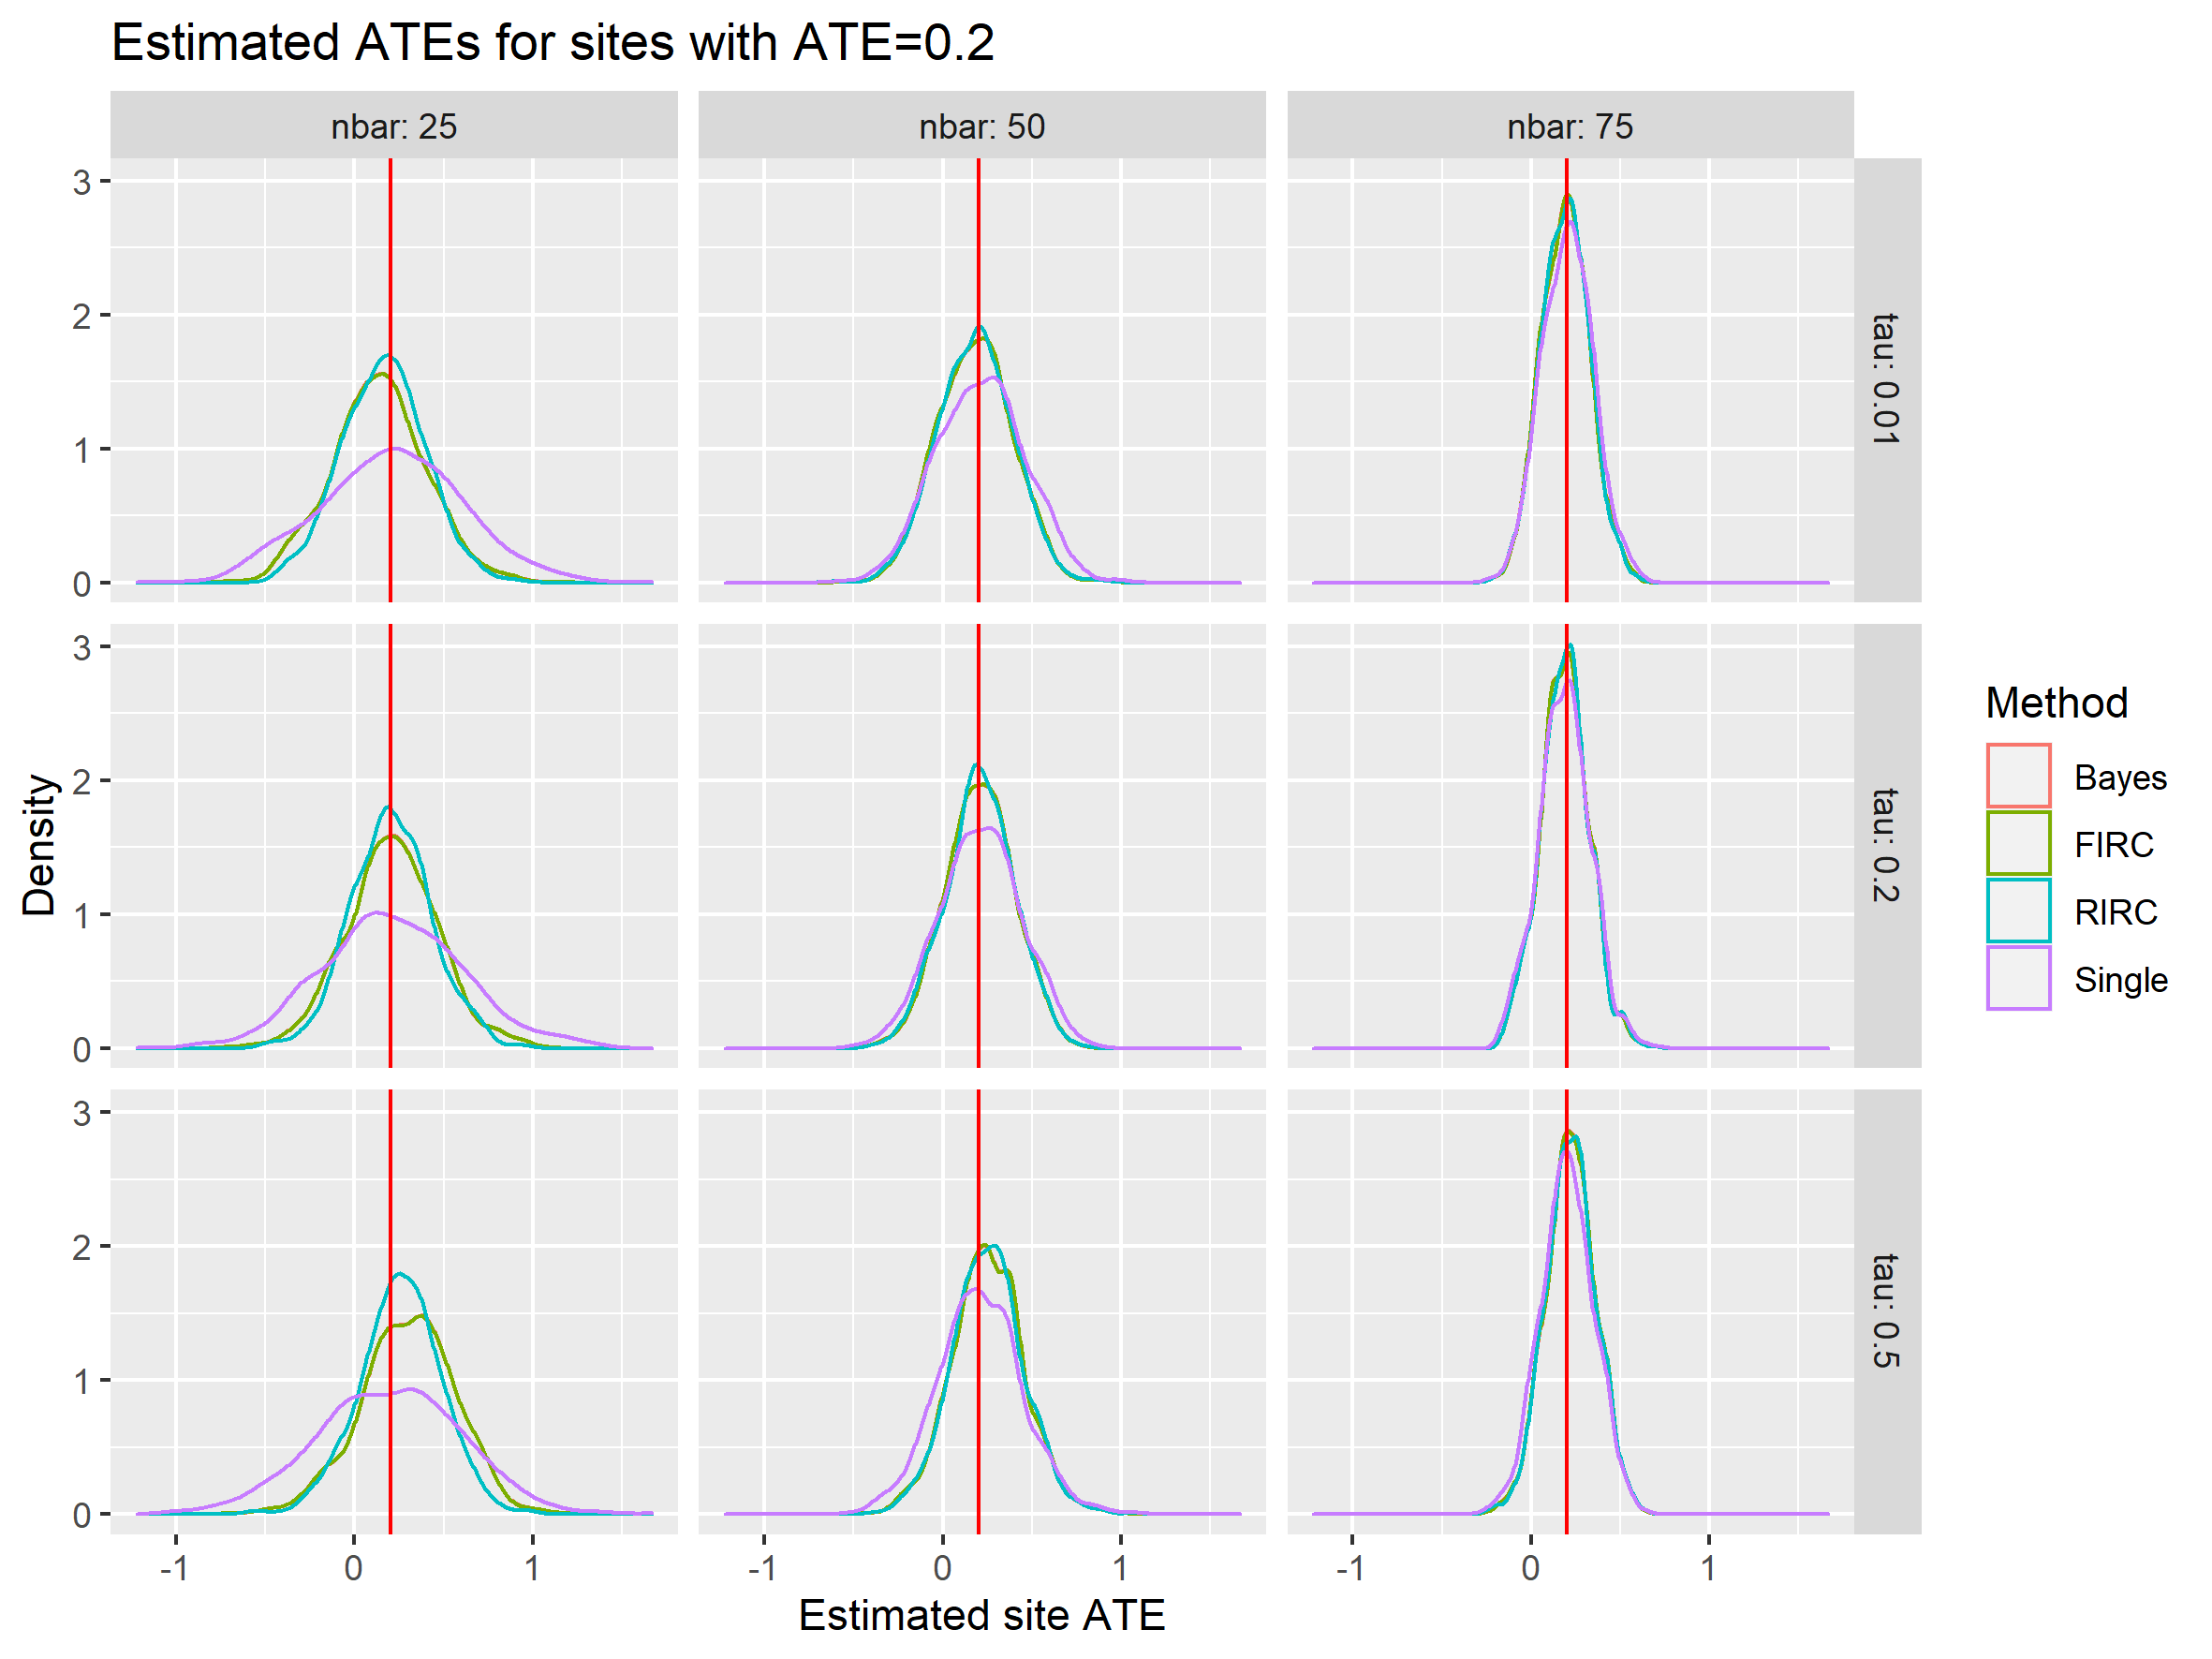
\includegraphics[width=\textwidth]{power_plot_ATE02_dens}
	\caption{Plot of power (at $\alpha = 0.1$) vs. true site ATE}
	\label{fig:power_plot_ATE02_dens}
\end{figure}


\subsection{Comparing MLMs with single-site estimates}

In this section, we compare the power of MLM estimates to the power of single-site estimates, i.e., the treatment-effect estimates for each site, ignoring the presence of any data from other sites.
We run single-site estimates using a standard Welch's t-test with pooled variances.

Figure \ref{fig:power_plot_comp} is the same as Figure \ref{fig:power_plot}, except the power curve for the single-site estimator is added on.
A few phenomena show up.
First, we note that MLMs reject either as or more frequently than their single-site counterparts, in all simulation settings.
The biggest difference in rejection rates occurs when $\bar{n}$ and/or $ICC$ are low.
In these low-information settings, MLMs have inflated type-I error rates for high values of $\tau$, but appear to have reasonable type-I error rates for low values of $\tau$ while maintaining increased power for values of $\tau_j$ that are greater than zero.

[Q: how to interpret? Low $\bar{n}$ means high standard errors. $ICC=0$ means all variation is residual, and not in site intercepts, i.e., higher standard errors.
This means that we can pool across sites super well, and do better?
This means that RIRC model has singular intercept fit (probably), and...]

\begin{figure}[ht]
	\centering
	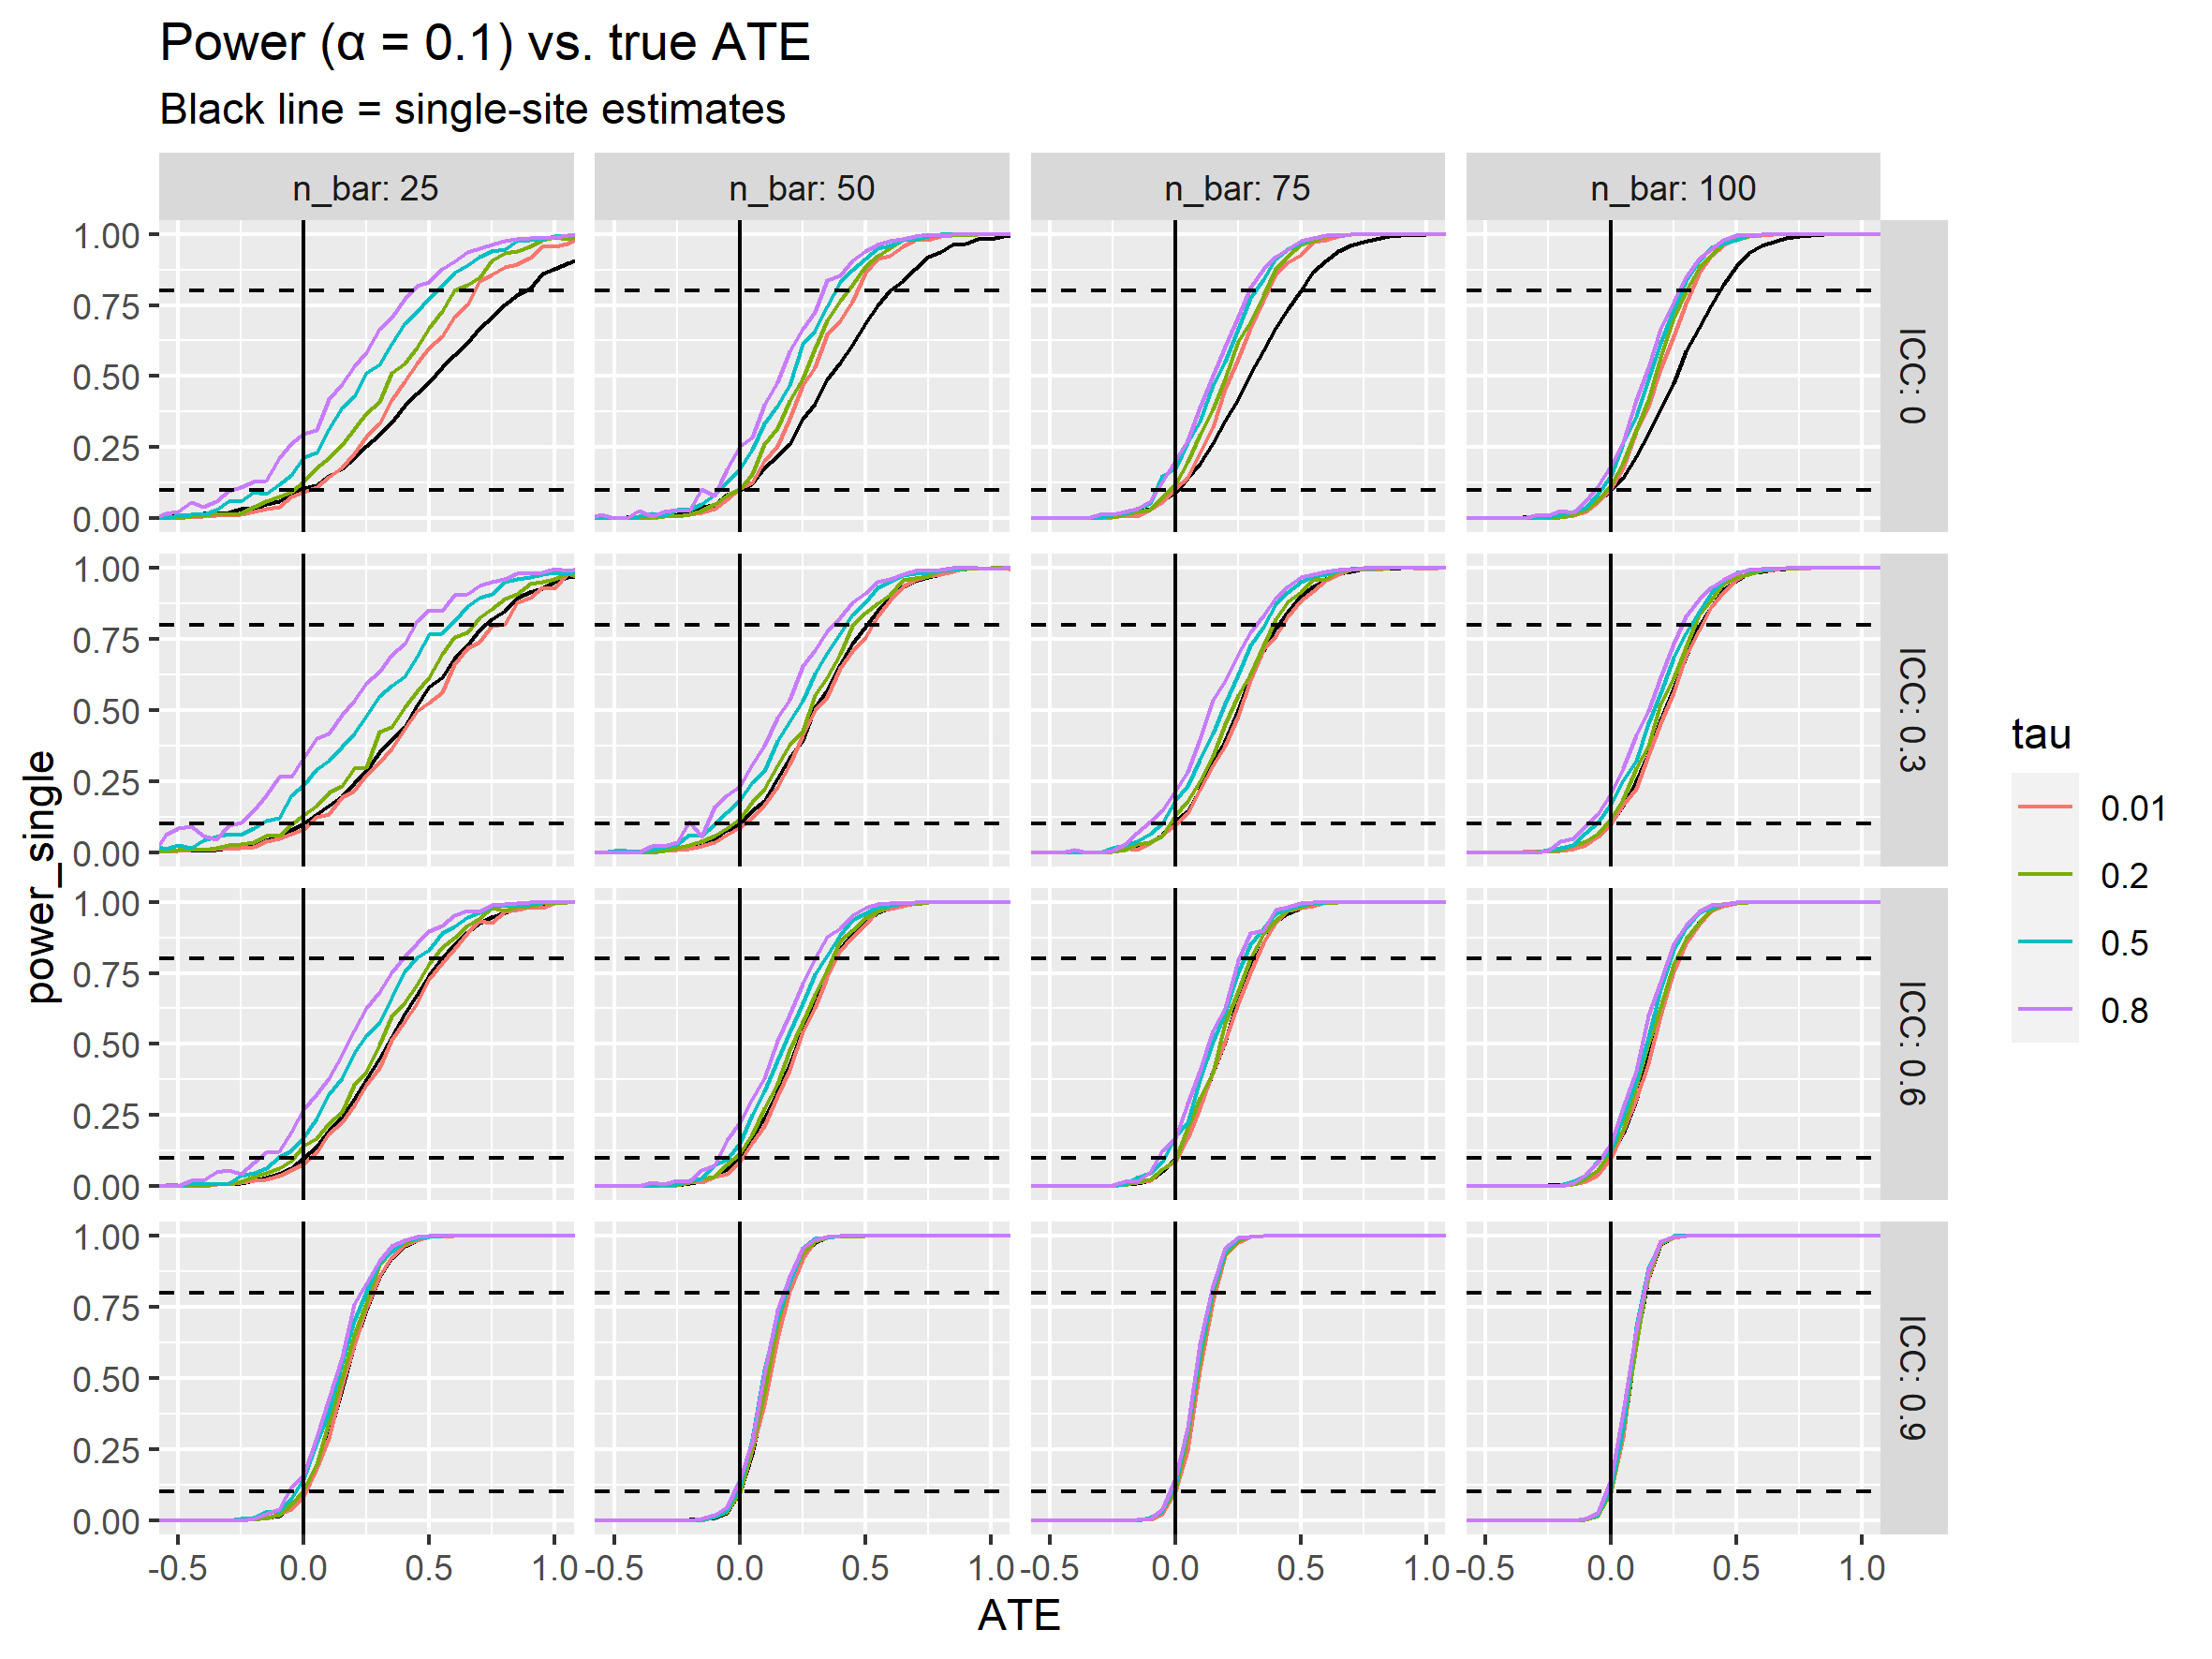
\includegraphics[width=\textwidth]{power_plot_comp}
	\caption{Plot of power (at $\alpha = 0.1$) vs. true site ATE}
	\label{fig:power_plot_comp}
\end{figure}

Figure \ref{fig:power_plot_comp_ATE02} is the same as Figure \ref{fig:power_plot_ATE02}, with the single-site estimates added in.
As expected, changing $\tau$ does not affect the single-site estimates.
[Note: this plot doesn't actually show much, perhaps we should remove it.]

\begin{figure}[ht]
	\centering
	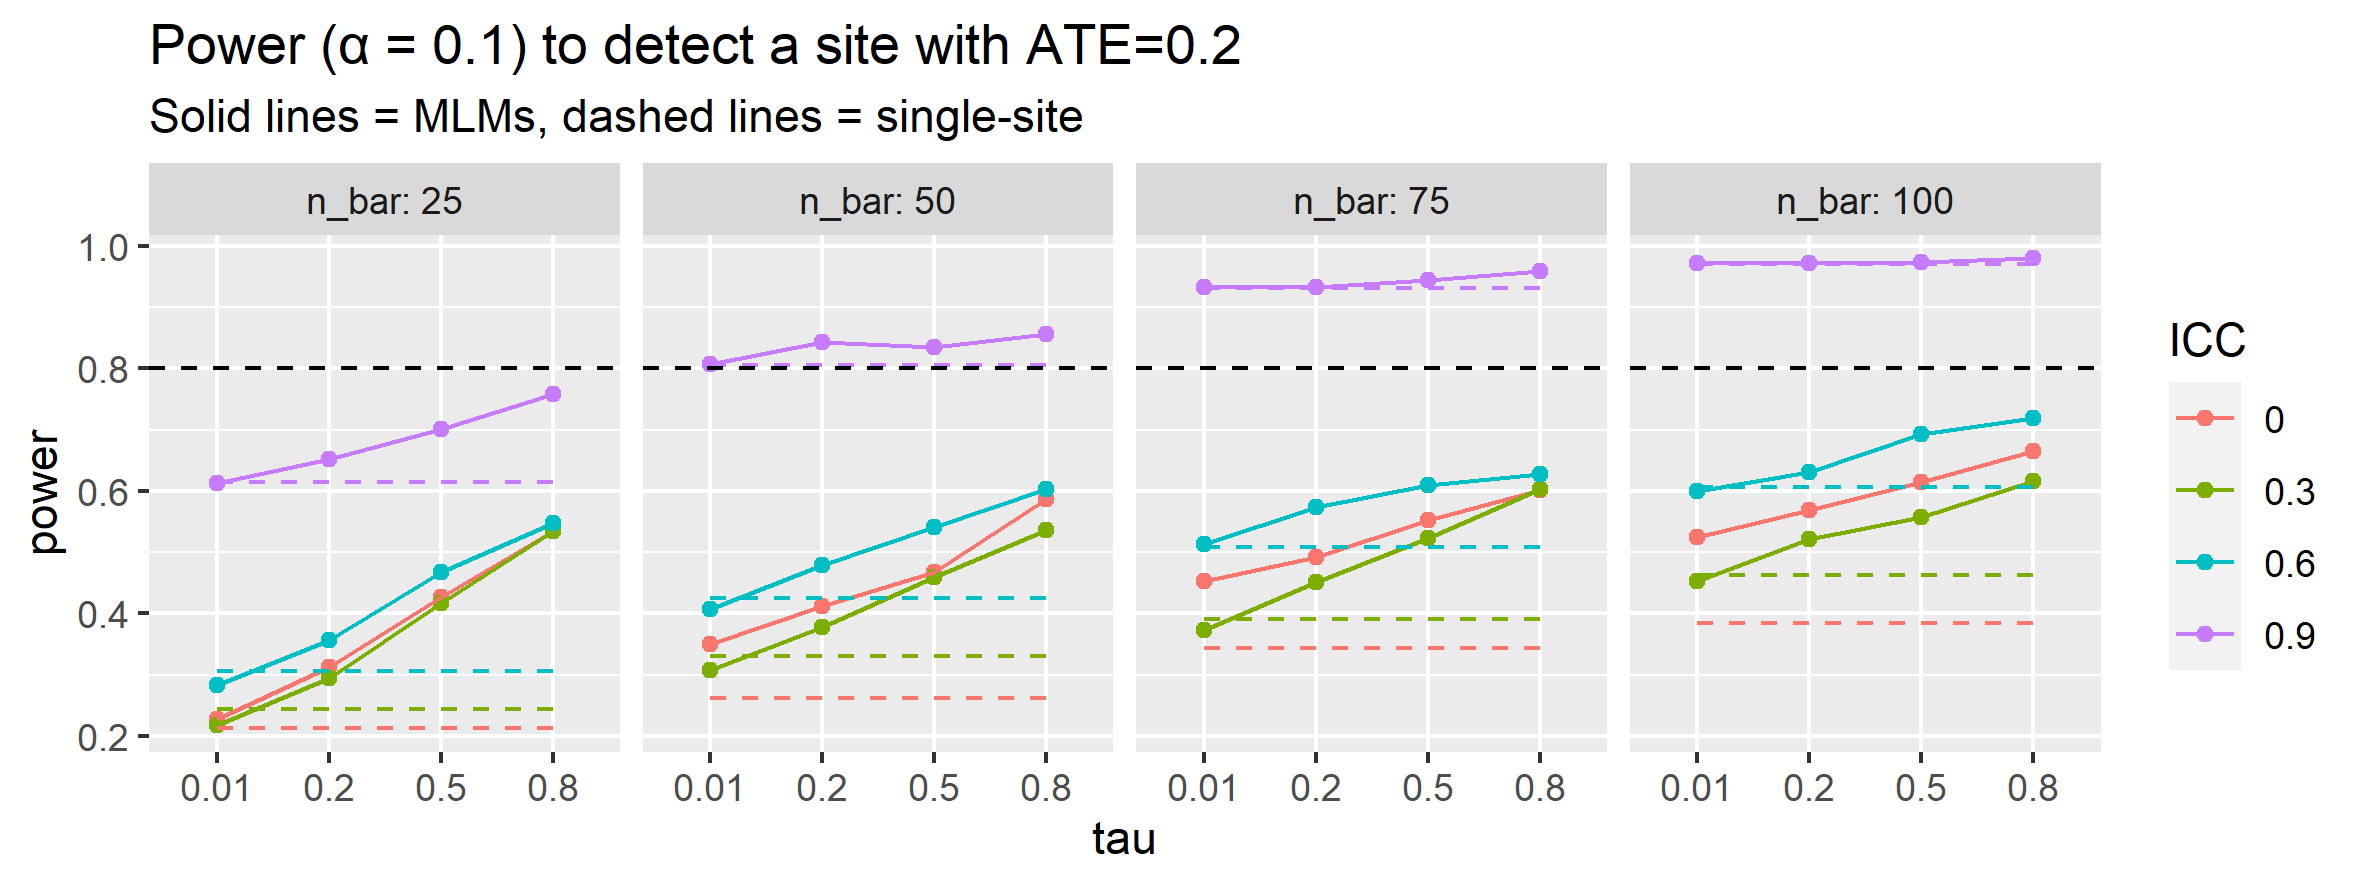
\includegraphics[width=\textwidth]{power_plot_comp_ATE02}
	\caption{Plot of power (at $\alpha = 0.1$) vs. true site ATE}
	\label{fig:power_plot_comp_ATE02}
\end{figure}

Finally, Figure \ref{fig:power_plot_comp_ATE02_dens} replicates Figure \ref{fig:power_plot_ATE02_dens}, except only including the $ICC = 0$ case.
We see that for sites with true $\tau_j = 0.2$, the MLM estimates are less spread than the single-site estimates.
[TODO: explain? This is a promising result, even if power isn't better, right?]
As $\tau$ increases, we also see the MLM estimates move toward the right, as expected with shrinkage.

\begin{figure}[ht]
	\centering
	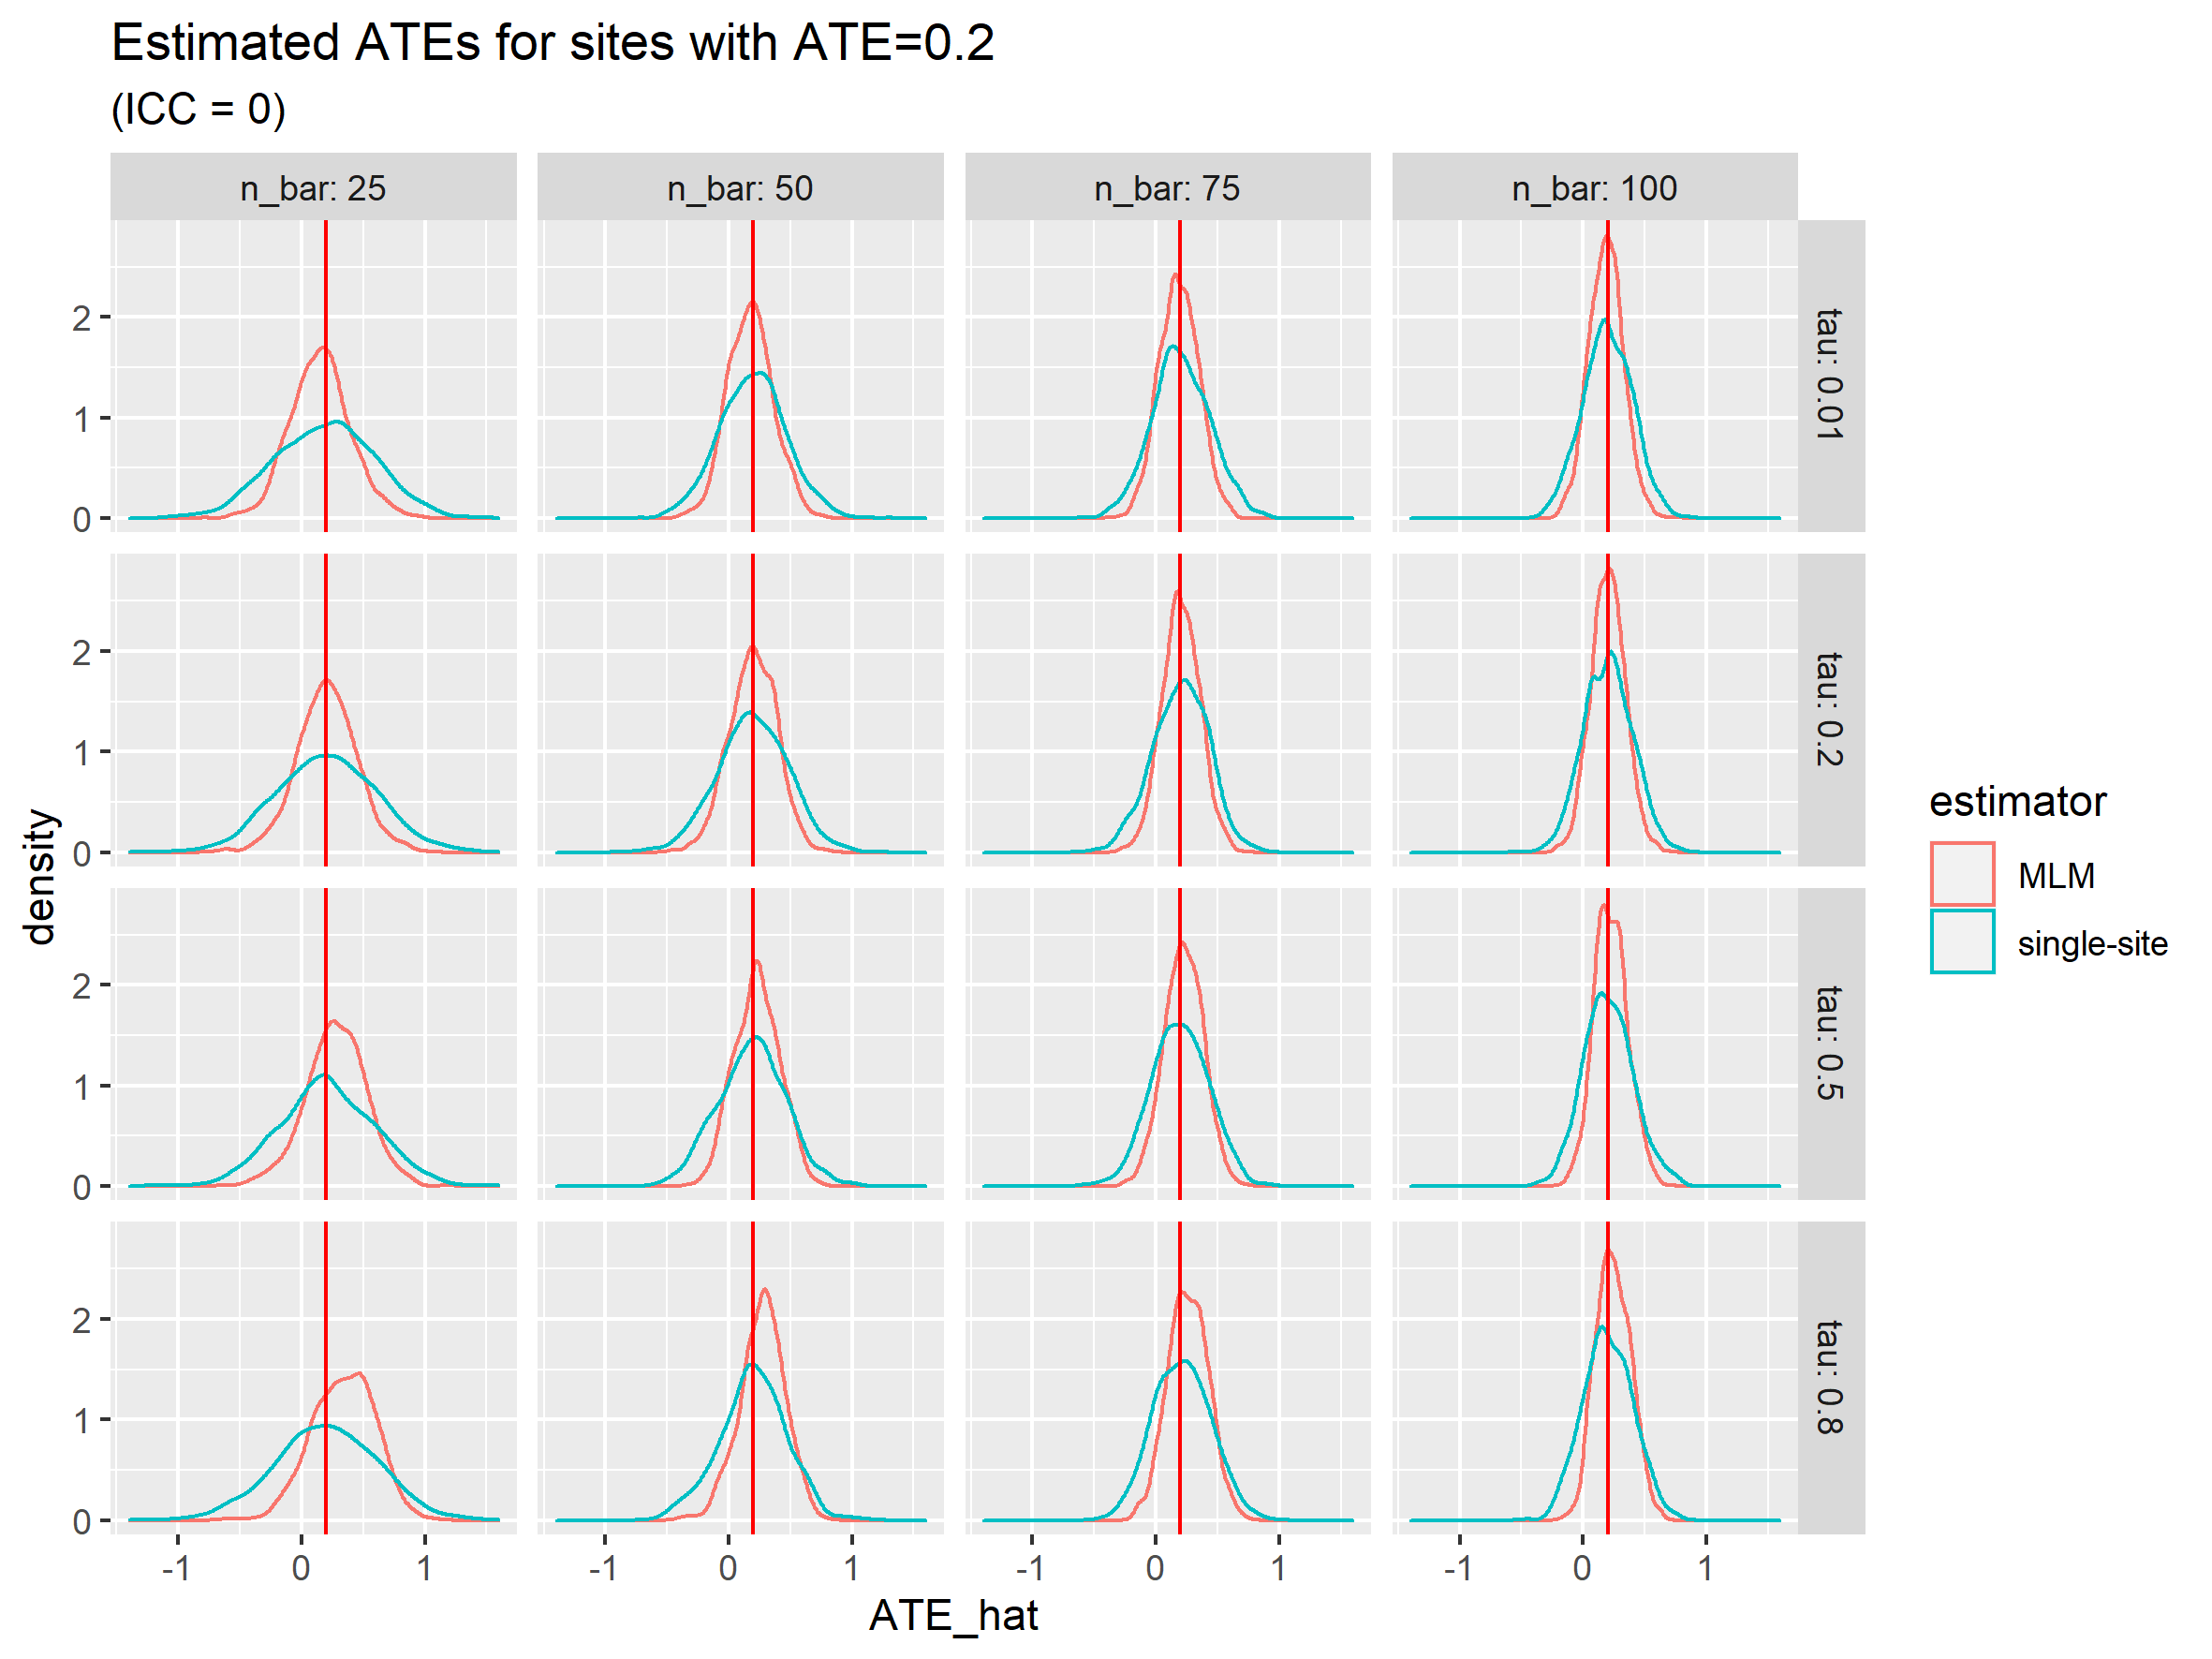
\includegraphics[width=\textwidth]{power_plot_comp_ATE02_dens}
	\caption{Plot of power (at $\alpha = 0.1$) vs. true site ATE}
	\label{fig:power_plot_comp_ATE02_dens}
\end{figure}

\appendix
\section{Appendix A: }

TODOs:
\begin{itemize}
	\item Singular fit rate analysis
	\item Show that rounding $\tau_j$ isn't a horrible sin
\end{itemize}
	
\end{document}